\documentclass[conference]{IEEEtran}
\usepackage{balance}
\usepackage{moreverb}
\usepackage{amsmath}
\usepackage[utf8]{inputenc}
\usepackage{pifont}
\usepackage{listings}  
\usepackage{color}  
\usepackage{textcomp}  
\usepackage{url}  
\usepackage{array}
\usepackage{booktabs}
\setlength{\heavyrulewidth}{1.5pt}
\setlength{\abovetopsep}{4pt}

\definecolor{listinggray}{gray}{0.98}  
\definecolor{lbcolor}{rgb}{0.98,0.98,0.98}  
\lstset{  
 backgroundcolor=\color{lbcolor},  
 tabsize=4,  
 rulecolor=,  
 language=java,  
        basicstyle=\scriptsize,  
        upquote=true,  
        aboveskip={1.5\baselineskip},  
        columns=fixed,  
        showstringspaces=false,  
        extendedchars=true,  
        breaklines=true,  
        showtabs=false,  
        showspaces=false,  
        showstringspaces=false,  
        identifierstyle=\ttfamily,  
        keywordstyle=\color[rgb]{0,0,1},  
        commentstyle=\color[rgb]{0.133,0.545,0.133},  
        stringstyle=\color[rgb]{0.627,0.126,0.941},  
}

\ifCLASSINFOpdf
   \usepackage[pdftex]{graphicx}
\else
\fi


\addtolength{\textwidth}{2mm}
\hyphenation{op-tical net-works semi-conduc-tor}

\begin{document}
\title{A Data Sharing and Synchronization Middleware Platform for Heterogeneous Medical Image Archives\vspace{-33pt}}

\author{\IEEEauthorblockN{Pradeeban Kathiravelu}
\IEEEauthorblockA{INESC-ID Lisboa\\
Instituto Superior T\'{e}cnico, Universidade de Lisboa\\
Lisbon, Portugal\\
Email: pradeeban.kathiravelu@tecnico.ulisboa.pt}\\[-5.0ex]
\and
\IEEEauthorblockN{Ashish Sharma}
\IEEEauthorblockA{Department of Biomedical Informatics\\
Emory University\\
Atlanta, Georgia, USA\\
Email: ashish.sharma@emory.edu}
\\[-5.0ex]}
\maketitle

\begin{abstract}
Big data science has more consumers and fewer producers of data. Scientific data is getting larger and larger and consists of a varying degree of heterogeneity in its content and storage media. Medical image archives are populated by the images and meta data by a few source providers and are read through different interfaces. With the growing adaptation of pervasive computing into medical domain and increasingly open access to data, the meta data stored in legacy data stores is shared and synchronized across multiple devices and users. With the increasing complexity of the image hierarchies, consumers of medical images should be able to bookmark and share the pointers to the sets of images and meta data from different sources. 

While many medical image sources provide APIs for public access, an architecture that permits an effective sharing and synchronization of meta data across multiple users, from different storage media, is still lacking. This paper presents \textit{MEDIator}, a data sharing and synchronization middleware platform for heterogeneous medical image archives. \textit{MEDIator} allows sharing pointers to data effectively, while letting the consumers manipulate the pointers without modifying th raw data. \textit{MEDIator} has been implemented for multiple data sources, including Amazon S3, The Cancer Imaging Archive (TCIA), caMicroscope\footnote{http://imaging.cci.emory.edu/camicroscope/}, and meta data from CSV files for cancer images.
\end{abstract}

\IEEEpeerreviewmaketitle

\section{Introduction}
Data sources contain data of different granularity. Data is organized in a hierarchical structure, where different levels are used to present data in specific formats. Folders and documents make a good example of this. Data units are often indexed with a unique identifier. A search across the data source would present the user with the list of matching criteria. Interesting sub set of the matching criteria may be bookmarked by the user and shared with others. Medical image archives have a hierarchy of information with a well-structured schema. Hence, medical image information can be retrieved at different granularity by the users, exploiting this hierarchy.

Sharing data among the consumers can be achieved by sharing pointers to the data, which reduces the redundancy and increases the efficiency of sharing and accessing the data as data duplication is minimized. Replica set is a pointer to stored data, which is created by the users as a bookmark, by choosing a sub set of data items that matches a search query or a specific user-defined criteria. Users can create replica sets with unique identifiers, and share their replica sets with other users and duplicate the replica sets, and update or delete their replica sets later. Hence, replica sets can be used as a way of tracking and sharing information. As heterogeneous data sources have different interfaces, a generic data replication and synchronization tool will be convenient, with sharing of replica sets from the data sources. 

In-memory data grids distribute storage and execution over multiple physical nodes, while giving a logically centralized view of a larger resource pool. An in-memory data grid can be an alternative for a traditional storage for the replica sets, as it will provide faster storage and access. Infinispan is a Java in-memory NoSQL store with implementations of distributed executor framework and MapReduce~\cite{infinispan}, which also has an actively maintained Android version. A deployment architecture consists of in-memory key-value stores such as Infinispan for sharing medical images will be scalable and pervasive.

While sharing data is encouraged in science~\cite{szala2006science}, algorithms and architectures should be designed for mashing up and making the public data sharing easy and effective. This paper presents the research and prototype implementations of $MEDIator$, a replication and data synchronization platform, exploiting the in-memory data grid projects, while consuming data sources such as TCIA via their public APIs. In the remaining of the paper, we will discuss the preliminary background information on $MEDIator$ in section II. Section III discusses solution architecture of $MEDIator$, where Section IV further presents the prototype implementation details of $MEDIator$. Section V closes the paper with conclusions and future work.

%
\section{Related Work}
%\subsection{Medical Image Archives}
%\paragraph*{\textbf{Medical Image Archives}}

Medical image archives often follow a well-defined hierarchy of images with different granularity. TCIA public API provides methods to retrieve the images and meta data of different granularity~\cite{prior2013tcia}, as shown by Figure~\ref{fig:methods}. These methods are invoked by the public APIs such as the REST API. An initial search on TCIA may contain parameters such as modality, in addition to collection name, patient ID, study instance ID, and series instance UID. Each of the searches in TCIA returns the output in a finer granularity.

\begin{figure}[!h]
	\begin{center}
		\resizebox{0.8\columnwidth}{!}{
			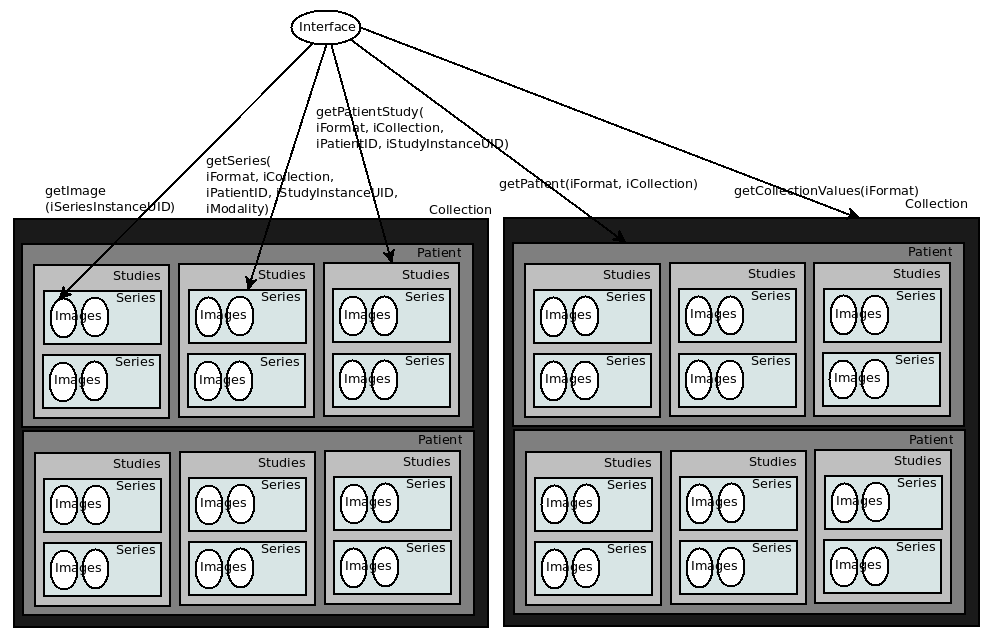
\includegraphics[width=0.8\textwidth]{methods.png}
		}
\vspace{-10pt}

	\end{center}
	\caption{Retrieving images and meta data}
	\label{fig:methods}
\vspace{-15pt}
\end{figure}


\paragraph*{\textbf{In-Memory Data Grids}}
In-memory data grids are extensively used in industry and academia, to provide a scalable memory and execution platform. Many commercial and open source in-memory data grid platforms exist. Infinispan and Hazelcast~\cite{hazelcast} are two commonly used open source in-memory data grids. Infinispan is often cited in researches~\cite{palmieri2012integrated,rosa2011goal,ruivo2011exploiting}.

\paragraph*{\textbf{Data Access and Integration}}
OGSA-DAI is a middleware platform that provides seamless integration and access to heterogeneous data sources~\cite{antonioletti2005design}. WS-DAI family of specifications provide a data access integration for web services~\cite{antonioletti2006ws}. While there are data sources integration platforms, a compact platform for medical image archives to share content across multiple users with light-weight pointers without actually duplicating the original content is still lacking.


\section{Solution Architecture}

Multiple nodes running Infinispan are leveraged and configured to create a cluster of $MEDIator$. Having multiple instances running over different nodes provide fault-tolerance, as when one node crashes or fails, the other nodes have the backup replica of the partitions stored in the terminated node. Figure~\ref{fig:deployment} depicts a higher level deployment view, with $MEDIator$ configured to execute over multiple physical nodes.
\begin{figure}[!h]
\begin{center}
 \resizebox{0.6\columnwidth}{!}{
  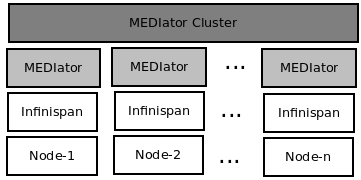
\includegraphics[width=0.6\textwidth]{deployment.png}
 }
\end{center}
 \caption{Deployment}
 \label{fig:deployment}
 \vspace{-18pt}
\end{figure}

When the user performs searches for the images, series, collections, and the other meta data, the results will be returned to the user, and the user can chose a subset of the returned results to create and store a replica set in  the Infinispan maps. A search query may contain different parameters that can define the scope of the search and the outcomes, and often return the outputs in a finer granularity. $MEDIator$ lets the users to create, update, retrieve, and delete replica sets, and share the replica sets with others.

When a sub set of such information is chosen and stored as a replica set, it is sufficient to store the unique identifiers of the matching data units of finer granularity than the original search query, as it would be sufficient to reproduce the data that is represented by the replica set. Hence, when using TCIA as the data source, storing an array of patient ID would be sufficient to identify the selected sub set of the collection including the array of patients. Similarly an array of study instance UID is sufficient to represent the selected sub set of any patient, and an array of series instance UID is sufficient to represent the selected sub set of any study, as it will contain an array of series. Hence $MEDIator$ stores the relevant IDs for the respective replica sets.

\subsection{Public APIs}
$MEDIator$ consists of 3 APIs, to be able to connect to specific data source, to integrate multiple data sources and meta data into the system, and to create replica sets for the data sources. Integrating with the data sources for data retrieval is done by $InterfaceAPI$, which is often provided by the remote data sources, as a mean to query and retrieve the raw data.

Methods for RESTful invocations are designed for each of the interfaces defining the APIs. Methods that are defined in the interfaces should be implemented by the classes that implement these interfaces. Table~\ref{table:interfaces} depicts the methods defined for each of the interfaces.

\begin{table}[!ht]
\centering
\caption{Methods defined for the Interfaces \vspace{-13pt}}
\label{table:interfaces}
\begin{tabular}{|c||c| |c|}

\toprule
\textbf{Data Source Management} & \multicolumn{2}{c}{\textbf{ReplicaSet Management}} \\
\midrule

\textbf{$InterfaceAPI$} & \textbf{$PubConsAPI$}&\textbf{$Integrator$} \\
\hline
retrieve & createReplicaSet&updateExistenceInDataSource \\
  & duplicateReplicaSet&doesExistInDataSource\\
  & getRawData&getRawData\\
 & getReplicaSet&getMetaData \\
 & putReplicaSet&putMetaData \\
 & updateReplicaSet&updateMetaData \\
 & deleteReplicaSet&deleteMetaData \\
\bottomrule
\end{tabular}
 \vspace{-13pt}
\end{table}

$PubConsAPI$ and $Integrator$ provide replica set management. $Integrator$ integrates multiple heterogeneous data sources into $MEDIator$ and provides a meta map and maps for each of the data sources to access the relevant information for each of the entry in a coarse granularity. $PubConsAPI$ provides and manages replica sets for each specific data source.  
%$InterfaceAPI$ provides data retrieval from the data source.

\paragraph*{DataProSpecs - PubConsAPI}
$DataProSpecs$ extends $PubConsAPI$ to design and implement the logic of replica sets management. The methods of $DataProSpecs$ can be invoked by knowing the respective ID of the replica set and the user ID of the user who owns the replica set. User ID is an identifier such as a user name or a `secret' or pass from the user. user IDs serve as the keys of the userReplicasMap. 

$createReplicaSet()$ requires the userID along with the elements to be stored in the replica set. It returns the $replicaSetID$, which is further used to uniquely identify the replica set. $getReplicaSet()$ requires only the relevant $replicaSetID$ to return the respective replica set. Similarly, $updateReplicaSet()$ requires $replicaSetID$ as well as the elements to be stored in the $replicaSet$, replacing the previous elements. $deleteReplicaSet()$ requires both the $userID$ and $replicaSetID$. Similarly, $duplicateReplicaSet()$ requires both $replicaSetID$ and the userID of the user to whom the replicaSet is shared to. Creating, deleting, and duplicating a replication set requires modification to the user replicas map, which holds the list of the replica sets for the particular user. Hence the necessity to input the userID. ReplicaSetID is a large number that can be randomly generated.
%It can be safely assumed to be harder to guess. Hence, this model is assumed to provide adequate security for this prototype.

\subsection{Integration with Data Sources}
Clinical data is deployed in multiple data sources such as TCIA, caMicroscope, and Amazon S3. Figure~\ref{fig:dsdeployment} depicts the deployment of the system with multiple data sources. A set of clinical data was uploaded to S3, where the meta data mapping of patientID \ding{213} fileName was available as a CSV file. Similarly CSV file depicting clinical information is available, as multiple properties against the UUID, such as patient ID. These files are parsed and stored into meta data maps in Infinispan. The CSV files containing meta data or $resource ID \ding{213} fileName$ mapping are stored locally in the file system or in a remote repository.
\begin{figure}[!htbp]
\begin{center}
 \resizebox{\columnwidth}{!}{
  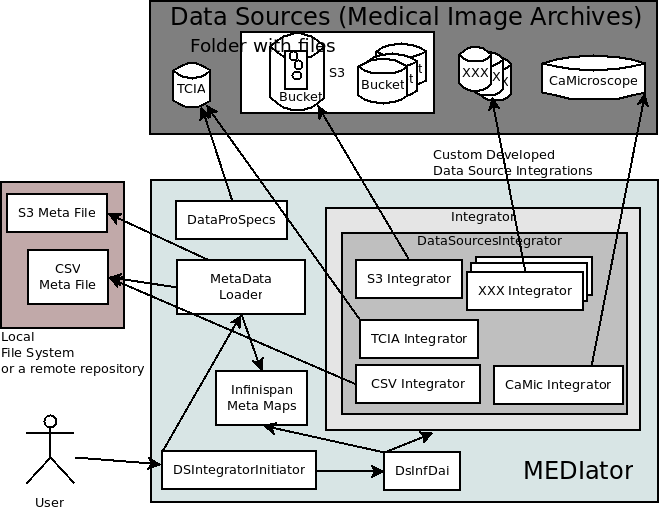
\includegraphics[width=\textwidth]{dsdeployment.png}
 }
\end{center}
 \vspace{-13pt}
 \caption{Deployment Diagram of the System and the Data Sources}
  \vspace{-13pt}
 \label{fig:dsdeployment}
\end{figure}

Each data source is connected to $MEDIator$ by implementing a class that extends Integrator interface. $DatasourcesIntegrator$, an abstract class provides the common features for the data sources integration. $CsvIntegrator$, $CaMicIntegrator$, $S3Integrator$, and $TciaIntegrator$ respectively function as the integrators for $CSV$, $caMicroscope$, $Amazon S3$, and $TCIA$. Further data sources can be integrated into $MEDIator$ by extending $DataSourcesIntegrator$ with a relevant sub class.$MetaDataLoader$ loads the CSV files and stores them into Infinispan maps, against the ID, such as the patient ID. 

A sub class of $InfDataAccessIntegration$, $DSInfDai$ holds the instances of map to store all the meta data. $DSIntegratorInitiator$ invokes the instances of $DSInfDai$, $MetaDataLoader$ and the other respective classes to parse the meta data, and store the instances into the respective maps. 

\subsection{$MEDIator$ Data Structures}
Infinispan distributed cache instances are created in $InfDataAccessIntegration$ as the data structures to hold the replica sets for each of the users. $userReplicasMap$ provides a mapping of userIdentifier \ding{213} array of replicaSetIDs. Hence, $userReplicasMap$ provide a listing of all the replica sets for the given user. replicaSetsMap is a mapping of replicaSetID \ding{213} replicaSet. A meta map provides a  mapping of replica set ID against a boolean array. The boolean value is set to true if the data source represented by the index of the boolean element in the array is available in the considered replica set.


\begin{lstlisting}  
    protected static Cache<String, Boolean[]> metaMap; /*csv, ca, tcia, s3*/
\end{lstlisting} 

The $metaMap$ stores a binary array against each of the key (such as, patientID) to point the existence of meta data in the data sources defined. Further, meta maps such as $tciaMetaMap$, $csvMetaMap$, $s3MetaMap$, and $caMetaMap$ are defined for each data source, against the replica set ID. $s3MetaMap$ provides the file name for the respective ID, which can be used to find the location of the file as it follows the pattern of of $S3\_BASE\_URL + folderName + ``/'' + fileName$. Similarly, $caMetaMap$ stores the URL that the respective object is stored. $csvMetaMap$ contains the meta data loaded from the CSV files against the respective ID. $tciaMetaMap$ stores a boolean array against the replica set ID, where a $true$ for the array element in the map indicates that a meta data with specific granularity is stored in the replica set.

Methods for updating, creating, and deleting meta data from these maps are available where creating or deleting meta data will update the availability to true/false for the respective index in the $metaMap$. $XXX\_META\_POSITION$ defines the position in the metaMap, where XXX stands for data sources such as CSV, CA, TCIA, and S3. Updating the existence will flop the respective boolean value for the entry. The $metaMap$ ensures easy indexing, and helps to search which of the data sources contain the respective information for any given key, such as a given patient ID. Similarly, data sources with a hierarchy such as $TCIA$ follow the same model, with a boolean array stored against each replica set ID at the top level.

\paragraph*{multi-tenancy}
$MEDIator$ is multi-tenanted, and it is aware of the multiple tenants or users using the system. All the users co-exist without the knowledge of existence of the other users, sharing the same cache space. 

\paragraph*{Access Logging}
Involving a time stamp for the class extending $PubConsAPI$, downloaded items can be tracked, and the diffs can be produced for the user download. Hence, a download can be paused and resumed later, downloading the images that have not been downloaded yet.

\paragraph*{Security}
$MEDIator$ can be further secured with user authentication. SAML tokens can be created for user names and passwords with the membership information, which can be validated later. This is designed as an Integrator for the Single Sign-on (SSO), as it involves multiple data sources. A create and validate API with user stores such as LDAP or OpenID should be designed and implemented, extending $MEDIator$.

\subsection{Software Architecture}
Figure~\ref{fig:arch} depicts the architecture of $MEDIator$, showing its components and dependencies. Dependencies are used unmodified. Apache HTTP Client and Mashape Unirest are configured and leveraged by the $InterfaceAPI$, to query and retrieve the raw data from the data sources. Infinispan, as the core dependency, is configured and exploited as the shared storage and distributed execution medium. Presentation layer dependencies such as Embedded Tomcat, Apache Velocity, and Log4j2 facilitate prototype application development with web pages, and configurable logging. Apache Maven is used as the project management dependency to build, deploy, and execute the project.
\begin{figure}[!htbp]
\begin{center}
 \resizebox{\columnwidth}{!}{
  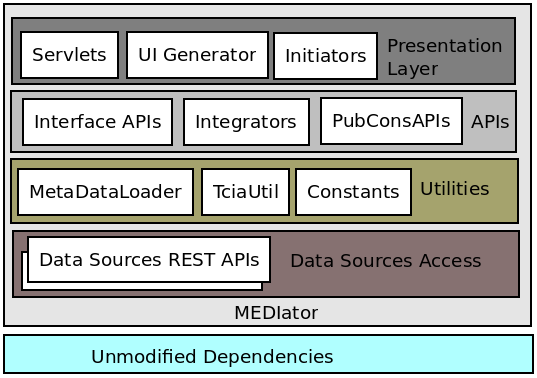
\includegraphics[width=\textwidth]{arch.png}
 }
\end{center}
  \vspace{-18pt}
  
 \caption{Architecture}
 \label{fig:arch}
 \vspace{-13pt}
 
\end{figure}


Data sources access layer consists of means of accessing the data sources, such as querying and downloading the data stored in Amazon S3 or TCIA, via the REST API. Utilities such as MetaDataLoader and TciaUtil provide utility methods and functionalities throughout the execution. InterfaceAPIs, Integrators, and PubConsAPIs are implemented at the top level, extending their respective base classes. The presentation layer consists of the Initiators that function as the starting point of the prototype applications. Servlets and UI Generators generate the presentation layer. 

Replica sets management is handled by both $Integrator$ and $PubConsAPI$ interfaces. If multiple data sources should be managed consecutively, having maps pointing to meta data from heterogeneous sources, $Integrator$ interface should be implemented in a class with the respective distributed maps to hold the meta data. If a single data source is involved with a fine grain control over a data source, it is sufficient only to extend and implement $PubConsAPI$. $InterfaceAPI$ integrates the data sources with $MEDIator$, such that the relevant data can be queried, searched, manipulated, and downloaded. Hence, respective classes should implement this interface for each of the data source. 

%$getRawData(String key)$ method should be implemented in the classes implementing the $PubConsAPI$ and $Integrator$ interfaces to be able to download the raw data from the data sources such as TCIA, caMicroscope, or S3, for the given replica set, potentially using Java web start.

\section{Implementation}
Based on the design, $MEDIator$ was implemented as a data sharing and synchronization middleware platform for heterogeneous medical image archives. Different complex data sources require custom development extending the generic framework. As creating and customizing the replica set require a more specific data structure, further implementations are done, extending the core class hierarchy. %\footnote{The source code can be accessed from \url{https://bitbucket.org/BMI/datareplicationsystem}}. 

%\subsection{TCIA Implementation}
$InfDataAccessIntegration$ implements the PubConsAPI for publisher/consumer of data, where $InterfaceManager$ implements the $InterfaceAPI$ for the interface between the data source and $MEDIator$. Invoker classes extending the abstract class $InterfaceManager$, implement the respective data source integration to invoke these methods. 

$TciaInvoker$ extends $InterfaceManager$ to implement the interfacing layer between the TCIA data source and $MEDIator$. Meta data such as collections, patients, studies, and series are retrieved at different levels, though the default download manager of TCIA downloads the data in series level, composed of the images of the series in a single zip archive. While having the default userReplicasMap to contain the IDs of the replica sets for each user, the replica set itself is stored in multiple maps instead of a single replicaSets map, to provide an efficient storage and access.

$DataProSpecs$ extends the $InfDataAccessIntegration$ class. 5 maps are created as below to represent the replica sets.
\begin{lstlisting}  
    protected static Cache<Long, Boolean[]> tciaMetaMap;
    protected static Cache<Long, String[]> collectionsMap;
    protected static Cache<Long, String[]> patientsMap;
    protected static Cache<Long, String[]> studiesMap;
    protected static Cache<Long, String[]> seriesMap;
\end{lstlisting} 

$tciaMetaMap$ contains a boolean array, which reflects which of the granularity of meta data is selected as a whole. For TCIA, if a few collections are selected, the first element of the array is set to true, and similarly, the other meta data are marked to true or false as shown by the below code segment.
\begin{lstlisting}  
        Boolean[] metaMap = new Boolean[4];
        metaMap[0] = collection != null;
        metaMap[1] = patientID != null;
        metaMap[2] = studyInstanceUID != null;
        metaMap[3] = seriesInstanceUID != null;

        putReplicaSet(replicaSetId, metaMap);
\end{lstlisting} 
The name of the collections, patientID, studyInstanceUID, and seriesInstanceUID are stored against the respective replicaSetID in collectionsMap, patientsMap, studiesMap, and seriesMap respectively. Hence changes are done at the respective maps. Duplicating the replicaSets duplicate the contents of the entire row to a new replicaSetID. Similarly, deleting a replicaSet deletes the respective information from all the maps.



\paragraph*{\textbf{Prototype Web Application and Evaluation}}
A prototype web application was built with $MEDIator$ architecture. Apache Velocity was used to generate the web pages for the replication tool. Apache Tomcat (Embedded) was integrated into the program such that it will get the user inputs from the HTML pages and present the output in pages formatted by Apache Velocity Templates. Respective servlets were created inside the servlets package to receive the inputs from HTML pages to the backend Java code.

A cluster with 6 identical nodes (Intel(R) Core(TM) i7-2600K CPU @ 3.40GHz and 12 GB memory) was used for evaluations. With synchronous backups enabled, $MEDIator$ showed a fault-tolerant behavior when a node failed and/or rejoined later. The time to initialize $MEDIator$ remained constant, regardless of the underlying data sources.


\section{Conclusion}
\balance

$MEDIator$ is a platform providing an ubiquitous access to medical meta data from the image archives, while providing fault tolerance and load balancing, leveraging the distributed shared memory platforms. A prototype has been implemented with multiple data sources containing cancer images, with Infinispan as the in-memory data store.

Consumers download the data by searching the image repository using the browser. The information that the consumer is interested in, gets updated whenever the data producers update or add patient information. Further improvements to $MEDIator$ should enable automated downloads to the consumers. While $MEDIator$ focuses on medical image archives, the design can also be implemented for any other data types with an index available to query and structure them as replica sets.


%\small{ \paragraph*{\textbf{Acknowledgments}} This work was partially supported by the Google Summer of Code 2014 project, under the mentoring organization \textit{Biomedical Informatics, Emory University}.}

\begin{thebibliography}{1}
	\scriptsize{
		
\bibitem{infinispan}
Francesco Marchioni.
\newblock {\em Infinispan Data Grid Platform}.
\newblock Packt Publishing Ltd, 2012.

\bibitem{szala2006science} A. Szalay and J. Gray, 2020 Computing: Science in an exponential world, {\em Nature, vol. 440}, pp. 413-414, 2006.

\bibitem{prior2013tcia}
Prior, F. W., Clark, K., Commean, P., Freymann, J., Jaffe, C., Kirby, J., ... \& Marquez, G. (2013, July). TCIA: an information resource to enable open science. In {\em Engineering in Medicine and Biology Society (EMBC), 2013 35th Annual International Conference of the IEEE} (pp. 1282-1285). IEEE.

\bibitem{hazelcast} Johns, M. (2013). {\em Getting Started with Hazelcast}. Packt Publishing Ltd.

\bibitem{palmieri2012integrated} Palmieri, R., di Sanzo, P., Quaglia, F., Romano, P., Peluso, S., \& Didona, D. (2012, January). Integrated monitoring of infrastructures and applications in cloud environments. In {\em Euro-Par 2011: Parallel Processing Workshops} (pp. 45-53). Springer Berlin Heidelberg.

\bibitem{rosa2011goal}Rosa, L., Rodrigues, L., \& Lopes, A. (2011, November). Goal-oriented self-management of in-memory distributed data grid platforms. In {\em Cloud Computing Technology and Science (CloudCom), 2011 IEEE Third International Conference on} (pp. 587-591). IEEE.

\bibitem{ruivo2011exploiting} Ruivo, P., Couceiro, M., Romano, P., \& Rodrigues, L. (2011, December). Exploiting total order multicast in weakly consistent transactional caches. In {\em Dependable Computing (PRDC), 2011 IEEE 17th Pacific Rim International Symposium on} (pp. 99-108). IEEE.

\bibitem{antonioletti2005design} Antonioletti, M., Atkinson, M., Baxter, R., Borley, A., Chue Hong, N. P., Collins, B., ... \& Westhead, M. (2005). The design and implementation of Grid database services in OGSA-DAI. {\em  Concurrency and Computation: Practice and Experience, 17} (2-4), 357-376.

\bibitem{antonioletti2006ws} Antonioletti, M., Krause, A., Paton, N. W., Eisenberg, A., Laws, S., Malaika, S., ... \& Pearson, D. (2006). The WS-DAI family of specifications for web service data access and integration. {\em ACM SIGMOD Record}, 35(1), 48-55.
}
\end{thebibliography}

\end{document}


